\graphicspath{{./Undergrad_ODEs/}}

\section{Review of Undergrad. ODEs}

Undergraduate Ordinary Differential Equations, or Calculus 4, is mostly a blitz of various analytical methods for solving initial value problems for linear (and some special case non-linear) differential equations. 

In this section we will review the following methods:

\begin{enumerate}
\item Separable Equations
\item First-Order: Integrating Factor
\item Homogeneous vs. Nonhomogeneous Equations
\item Solving for Complementary Solutions
\begin{itemize}
\item Linear constant coefficient ODEs
\end{itemize}
\item Solving for Particular Solution:
\begin{itemize}
\item Undetermined Coefficients
\item Variation of Parameters
\end{itemize}
\item Bonus Methods and Conceptual Fun:
\begin{itemize}
\item Transform Methods (i.e., ``Euler" type, Ricatti type, etc)
\item Laplace Transforms
\item Non-Dimensionalization
\item Introduction to Dynamical Systems, e.g., systems of ODEs
\begin{itemize}
\item Eigenvalues and Systems of Linear Homogeneous ODE
\item The Matrix Exponential
\item Non-homogeneous Linear Systems
\item Non-linear Systems of ODEs
\end{itemize}
\end{itemize}
\end{enumerate}

Since undergraduate ODEs does not have much theory, we will try to motivate each method, when possible, otherwise sit back and enjoy the following stampede of methods!


%%%%%%%%%%%%%%%%%%%%%%%%%%%%%%%%
%
% SEPARABLE EQUATIONS
%
%%%%%%%%%%%%%%%%%%%%%%%%%%%%%%%%

\subsection{Separable Equations}

Perhaps the most natural method to solve ODEs comes from ideas of calculus, where we simply want to integrate anything and everything possible. The differential equations we are able to solve via pure integration are of the form, where you can \emph{separate} the dependent variable and indepedent variables entirely, i.e., if we have the following ODE to solve,
$$\frac{dy}{dx} = f(x,y) = g(x) h(y),$$ with $y(a) = y_a$ as initial data. 

We can then separate the equation, 

$$\frac{dy}{h(y)} = g(x) dx.$$

Now integrating  both sides we can get a functional relationship between $y$ and $x$. Unfortunately, sometimes this relationship is nonlinear or transcendental, making it difficult to write a solution like $y=y(x)$; however, we can still use the initial data to solve for the integration constant. 

For example consider, $$\frac{dy}{dt} = -y(1-y),$$ with $y(0)=2$. We can then go through the separation method to find,

\begin{align*}
\frac{dy}{y(1-y)} &= -dt \\
\int \frac{1}{y(1-y)} dy &= \int -dt \\
\log(y) - \log(1-y) &= -t + C \\
\frac{y}{1-y} =&= Ae^{-t} 
\end{align*}

and hence doing a little algebra we find that $$y(t) = \frac{Ae^{-t}}{1+Ae^{-t}}.$$

Now using the initial value information we can get $A$, 

$$y(0)=2 \Rightarrow 2 = \frac{A}{1+A} \Rightarrow A = -2.$$

Therefore our solution is $y(t) = \frac{-2e^{-t}}{1-2e^{-t}}.$ Note that this solution will blow up for finite time, namely when $e^{-t} = \frac{1}{2}$ or $t=\ln\left(\frac{1}{2}\right)$.




%%%%%%%%%%%%%%%%%%%%%%%%%%%%%%%%
%
% First-Order Integrating Factor
%
%%%%%%%%%%%%%%%%%%%%%%%%%%%%%%%%

\subsection{First-Order Integrating Factor}

The world would be very nice, but boring, if all first-order differential equations were separable. Note: Not all separable equations are useless $\rightarrow$ some describe many processes in population biology or black hole thermodynamics! \\

To simply make an equation not separable, we just need to tack on one extra term; however, we will restrict ourselves to linear first-order equations now of the form,

\begin{equation}
\label{1st_order_ode} \frac{dy}{dx} + p(x) y(x) = q(x),
\end{equation}

where we assume $p(x)$ and $q(x)$ are continuous. To solve the above equation we consider the left hand side of (\ref{1st_order_ode}) to be the result of a product rule. However, to make it such we need to multiply all the terms by fudge factor given in exponential form, also known as the \emph{integrating factor},

$$e^{\mu(x)}  = e^{\int p(x) dx},$$

thereby giving $\frac{d}{dx} e^{\mu(x)} = p(x) e^{\mu(x)}$ since $\frac{dv}{dx} = p(x).$ Doing so we see the product rule gives, 

$$\frac{d}{dx} \left[ e^{\int p(x) dx } y(x) \right] = e^{\int p(x) dx} \left[ \frac{dy}{dx} + p(x) y(x) \right] = e^{\int p(x) dx} q(x).$$

Hence to solve (\ref{1st_order_ode}), we need to integrate both sides and then easily solve for $y(x)$, e.g.,

\begin{align*}
\frac{d}{dx} \left[ e^{\int p(x) dx } y(x) \right] &= e^{\int p(x) dx} q(x) \\
\int \frac{d}{dx} \left[ e^{\int p(x) dx } y(x) \right] dx &= \int e^{\int p(x) dx} q(x) dx \\
e^{\mu(x) } y(x) &= \int e^{\mu(x) } q(x) dx
\end{align*}

and therefore we find that $$y(x) = e^{-\mu(x)}  \int e^{\mu(x)} q(x) .$$

\subsubsection{Example: Integrating Factor}

Let's do an example! Consider $$\frac{dy}{dt} +  \frac{1}{3} t^2 y(t) = t^2.$$

Using the integrating factor approach we first identity $e^{\mu(t)}$ as $$e^{\mu(t)} = e^{\int \frac{1}{3} t^2 dt } = e^{t^3}.$$

Then using the methodology developed above, we see $$y(t) = e^{-t^3} \int  e^{t^3} t^2 dt,$$

and hence $$y(t) = \frac{1}{3} + C e^{-t^3},$$ 

where $C$ can be solved using initial data.



%%%%%%%%%%%%%%%%%%%%%%%%%%%%%%%%
%
% Honogeneous vs. Non-homogeneous Equations
%
%%%%%%%%%%%%%%%%%%%%%%%%%%%%%%%%

\subsection{Homogeneous vs. Non-homogeneous Equations}

Before we begin our trajectory into higher order linear differential equations, we are going to set a clear discrepancy between homogeneous and non-homogeneous equations. In two words, a homogeneous equation is when we have a bunch of dependent variable stuff equal to zero, i.e., 

$$\hat{L}y(x) =  c_n(x) \frac{d^n y}{dx^n} + c_{n-1}(x) \frac{d^{n-1} y}{dx^{n-1}} + \ldots + c_2(x) \frac{d^2 y}{dx^2} + c_1(x) \frac{dy}{dx} + c_0(x) y = 0.$$

On the other hand a non-homogeneous equation looks like the above, except with non-zero right hand side, e.g., 

$$\hat{L}y(x) = c_n(x) \frac{d^n y}{dx^n} + c_{n-1}(x) \frac{d^{n-1} y}{dx^{n-1}} + \ldots + c_2(x) \frac{d^2 y}{dx^2} + c_1(x) \frac{dy}{dx} + c_0(x) y = q(x).$$

The reason we make clear the distinction is because if we consider a solution to the \emph{non-homogeneous} problem, call it $y_P(x)$, we have 

$$\hat{L} y_P(x) = q(x),$$ while a solution for the homogenous problem, call it $y_C(x)$, looks like $$\hat{L} y_C(x) = 0.$$

Therefore if we consider a combined solution, $$y(x) = y_C(x) + y_P(x),$$ we have

$$\hat{L} y(x) = \hat{L} y_C(x) + \hat{L} y_P(x)  = q(x).$$

Hence if we are trying to solve a non-homogeneous problem, we see it is \emph{necessary} to solve the homogeneous problem as well. We call the solution to the homogeneous problem the \emph{complementary} solution, while the solution to the non-homogeneous problem is called the \emph{particular} solution. \\

Furthermore we note that any scaling multiple of the complementary solution is also a problem to the homogeneous problem, i.e., $$\hat{L}[ \alpha y_C(x) ] = 0,$$

where $\alpha\in\mathbb{C}.$




%%%%%%%%%%%%%%%%%%%%%%%%%%%%%%%%
%
% Linear Constant Coefficient ODEs (2nd Order)
%
%%%%%%%%%%%%%%%%%%%%%%%%%%%%%%%%

\subsection{Linear Constant Coefficient ODEs}

We will discuss equations of the form, 

$$\hat{L}y(x) =  c_n \frac{d^n y}{dx^n} + c_{n-1} \frac{d^{n-1} y}{dx^{n-1}} + \ldots + c_2 \frac{d^2 y}{dx^2} + c_1 \frac{dy}{dx} + c_0y = 0,$$

where $\{ c_j \}_{j=0}^{n} \in \mathbb{R}.$ For equations of this form we will show that our solution technique assumes an ansatz for a solution and by doing so terms this differential problem into more an algebraic polynomial root-finding issue. We also note that since this is an $n^{th}$ order homogeneous equation, we need to find $n$ linearly independent solutions for our complementary solution.

To illuminate this idea better further, we will show the possibilities for second-order linear constant coefficient ODEs. 

We now consider the following ODE,
\begin{equation}
\label{2nd_order_cc_ode} a \frac{d^2 y}{dx^2} + b \frac{dy}{dx} + c y = 0,
\end{equation}

with initial data of the form $y(0) = y0$ and $y'(0) = y_0^P.$ We assume solutions of the following form $$y = e^{rt},$$ where $r\in\mathbb{C}$. Continuing with this path we see

\begin{align*}
a \frac{d^2 y}{dx^2} + b \frac{dy}{dx} + c y &= a \frac{d^2}{dx^2}\left[e^{rt}\right] + b \frac{d}{dx}\left[e^{rt}\right] + c \left[e^{rt}\right]\\
& = a r^2 e^{rt} + b r e^{rt} + c e^{rt} \\
& = e^{rt} \Big[ a r^2 + b r + c \Big] = 0
\end{align*}

and hence we now need to solve $$a r^2 + b r + c = 0,$$ and then will have the numeric values or $r$ to build our complementary solution. We call this polynomial the \emph{characteristic equation}. 

Moreover we note at this junction that we need $n$ linearly independent solutions for our complementary solution, and in the above we had a second-order linear ODE and obtained a second-order polynomial to find the roots of. In this second-order example, we will have three possible cases that the roots can fall into. Naturally this goes back to properties of quadratic equations and when there are real, complex, or double roots. 

We will highlight each case with an example. 

\begin{itemize}

%
% CASE 1
%
\item[Case 1]: $b^2 - 4ac > 0$ (real roots)

Consider the following example $$y'' -  y' - 2y = 0.$$

Substituting our ansatz, $y= e^{rt}$ we find we get the following algebraic equation to solve $$r^2 - r - 2=0.$$

Solving this equation we find that $r = \{ -1,2\}$ and hence we get two linearly independent solutions that solve the homogeneous problem above, $$\{ e^{-x}, e^{2x}\},$$

and so our complementary solution is $$y_C(x) = \alpha_1 e^{-x} + \alpha_2 e^{2x}.$$

%
% CASE 2
%
\item[Case 2]: $b^2 - 4ac < 0$ (complex roots)

Consider the following example $$y''+2y' + 2y = 0.$$

Again, substituting our ansatz, $y=e^{rt}$, we get the following characteristic equation $$r^2+2r+2=0.$$

Solving this equation we find $r = \{ 1-i,1+i\}$ and so our linearly independent solutions are $\{ e^{(1-i)x}, e^{(1+i)x}\}$. We can easily write the complementary solution as $$y_C(x) = \alpha_1 e^{(1-i)x} + \alpha_2 e^{(1+i)x},$$

but we will massage our solutions to a more friendly form! After much algebra, we find we can write the above as:

$$y_C(x) = e^{x} \Big[ \alpha_1 \cos(x) + \alpha_2 \sin(x) \Big.$$

In general if we find our complex roots to be $\{ a-bi, a+bi \},$ we can write our complementary solution as

$$y_C(x) = e^{ax} \Big[ \alpha_1 \cos(bx) + \alpha_2 \sin(bx) \Big].$$


%
% CASE 3
%
\item[Case 3]: $b^2-4ac = 0$ (root with multiplicity $> 1$.)

Consider the following example $$y'' - 6y' + 9y = 0.$$

Using our ansatz, $y=e^{rt}$, we obtain the following characteristic equation $$(r-3)^2 = 0.$$

Hence solving this equation we find that $r=3$ is a double root, i.e., a root with multiplicity $> 1$. Therefore if we tried to write our complementary solution is a similar way to \emph{Case 1}, we would have $$y_C(x) = \alpha_1 e^{3x} + \alpha_2 e^{3x} = \alpha ^{3x},$$

and thereby only have \emph{ONE} linearly independent solution, when we need two! The method we will employ to find this second solution is a special (easy) case of \emph{Reduction of Order}. We assume the second linearly independent solution $y_2(x)$ has the form $$y_2(x) = v(x)y_1(x) = v(x) e^{3x},$$ where $y_1(x) = e^{3x}$ is the linearly independent solution we do have!

Plugging this into the ODE we get,
\begin{align*}
y_2'' - 6y_2' + 9y_2 &= [v'' y_1 + 2v'y' + vy_1''] - 6[v'y_1 + vy_1'] + 9vy_1 \\
&= [v''y_1 +2v'y_1' - 6v'y_1] + v(x) [ y_1'' - 6y_1' + 9y_1] \\
&= v''e^{3x} + (3)2v'e^{3x} - 6v'e^{3x} \\
&= e^{3x} \Big[ v'' \Big] = 0 \\
\end{align*}

and therefore we need to solve $v'' = 0$ and find $v(x) = \beta x + \gamma.$ Hence our second linearly independent solution is $$y_2(x) = ( \beta x+\gamma)e^{3x},$$

and our complementary solution is

$$y_C(x) = \alpha e^{3x} + ( \beta x+\gamma)e^{3x} = ( \tilde{\alpha} + \beta x )e^{3x},$$

where $\tilde{\alpha} = \alpha+\gamma$, but is just another constant to be found using the initial data afterall, so it's nothing too fancy!

\end{itemize}



%%%%%%%%%%%%%%%%%%%%%%%%%%%%%%%%
%
% Solving for the particular solutions!
%
%%%%%%%%%%%%%%%%%%%%%%%%%%%%%%%%

\subsubsection{Solving for the Particular Solution}

In this section we are concerned with finding the particular solution, $y_P(x)$, for non-homogeneous equations. We will assume that we already found the complementary solution, i.e., the solution to the homogeneous equation, $y_C(x)$. We are concerned with the particular solutions of linear constant-coefficient equations, i.e., 

\begin{equation}
\label{nonhomogeneous_eq} c_n(x) \frac{d^n y}{dx^n} + c_{n-1}(x) \frac{d^{n-1} y}{dx^{n-1}} + \ldots + c_2(x) \frac{d^2 y}{dx^2} + c_1(x) \frac{dy}{dx} + c_0(x) y = q(x).
\end{equation}

Like in the previous section, we illustrate this concept with $2^{nd}$ order linear constant coefficient equations, $$c_2 y'' + c_1 y' + c_0 y = q(x).$$

We will describe two methods for finding the \emph{particular} solution,
\begin{enumerate}
\item Undetermined Coefficients
\item Variation of Parameters
\end{enumerate}

\begin{itemize}
%
% Undetermined Coefficients
%
\item {\bf{Undetermined Coefficients:}}

This method of finding a particular solution is similar to that of ``guess and check!". This method will only work for special cases of $q(x)$, namely if $q(x)$ belongs to the following families of functions $\{ a_n x^n +\ldots a_1 x+a_0, e^{ax}, \sin(ax),\cos(ax)\}$, or any products of those. 

\begin{itemize}
\item \emph{Example 1:} Consider the following example, $$y'' - y' - 2y = 6x^2.$$

Recall we found the complementary solution to be $y_C(x) = \alpha_1 e^{-x} + \alpha_2 e^{2x}.$ Now since $q(x)$ is a polynomial, we will assume a polynomial form for $y_P(x)$, i.e., we will let $y_P(x) = c_1 x^2 + c_2 x + c_3.$

Substituting our particular solution into the ODE gives
\begin{align*}
y''-y'-2y= 6x^2 &= \frac{d^2}{dx^2}(c_1 x^2 + c_2 x + c_3) - \frac{d}{dx} ( c_1 x^2 + c_2 x + c_3) - 2(c_1 x^2 + c_2 x + c_3) \\
&= (2c_1) - (2 c_1 x + c_2) - 2(c_1 x^2 + c_2 x + c_3) \\
&= [-2 c_1] x^2 - 2[ c_1 + c_2 ]x + [2c_1 - c_2 -2c_3] 
\end{align*}

Hence we see that we have the following system of equations to solve
\begin{align*}
-2 c_1 &= 6 \\
-2c_1 - 2 c_2 &= 0 \\
2c_1 - c_2 - 2c_3 &= 0\\
\end{align*}

Solving this system we find that $c_1 = -3$, $c_2 = 3$, and $c_3 = -\frac{9}{2}.$ Thereby making our particular solution $y_P(x) = -3x^2+3x-\frac{9}{2}.$ Hence our full solution to this non-homogeneous equation is
$$y(x) = y_C(x) + y_P(x) =  \alpha_1 e^{-x} + \alpha_2 e^{2x} + \Big[-3x^2+3x-\frac{9}{2}\Big],$$

up to using the initial data to solve for $\{\alpha_1,\alpha_2\}.$ \emph{Note} that even though $q(x)$ did not have a linear term of constant term, the particular solution did have those components. Hence we have to make sure to include all the polynomial terms at the same order and below as $q(x)$.
\end{itemize}

We can do a similar process if $q(x)$ takes on the other functional forms. Below is a table for what particular solution to ``guess" for each $q(x)$.

$$\begin{array}{|c|c|}
\hline 
{\bf{q(x)}}   & {\bf{y_P(x)}} \\
\hline
e^{ax}   & c_1 e^{ax}\\
\hline
\sin(bx) & c_1 \sin(bx) + c_2\cos(bx) \\
\hline
\cos(bx) & c_1 \sin(bx) + c_2\cos(bx) \\
\hline
\beta \sin(bx)+ \gamma \cos(bx) & \sin(bx) + c_2\cos(bx) \\
\hline
a_n x^n \ldots a_2x^2 + a_1 x + a_0 & c_n x^n \ldots c_2x^2 + c_1 x + c_0 \\
\hline
\end{array}$$

\begin{itemize}
\item \emph{Example:} Resonance

One other subtle point to make is in the case when $q(x) = e^{ax}$. If our complementary solutions are exponential functions, it is possible that our complementary solutions may already include a term of $e^{ax}$, i.e., $y_C(x) = \alpha_1 e^{ax} + \alpha_2 e^{bx}.$ In this case, we will have \emph{resonant} solutions. 

Our particular solution will then take on a term like $y_P(x) = c_1 x e^{ax},$ analogous to what we did in the case of multiple roots using Reduction of Order.

\end{itemize}


%
% Variation of Parameters
%
\item {\bf{Variation of Parameters:}}

The next method for finding particular solutions assumes we already know what the complementary solutions are. Like the last case, we will assume we are trying to solve a $2^{nd}$ order linear ODE. \emph{Note} this method does not only work for linear constant coefficient ODEs, unlike undetermined coefficients.  This method will work for higher order equations analogously (the algebra just gets a \emph{bit} more undesirable).

Called, \emph{variation of parameters}, it is a method that exploits a more general \emph{reduction of order} technique. We begin with the set of fundamental solutions $\{ y_1(x), y_2(x) \}$, i.e., where $y_C(x) = \alpha_1 y_1(x) + \alpha_2 y_2(x).$ We now assume the particular solution takes a reduction-of-order-form,
\begin{equation}
\label{vop_form} y_P(x) = u_1(x) y_1(x) + u_2(x) y_2(x),
\end{equation}

where $\{ u_1(x), u_2(x) \}$ are unknown functions that we now set out to find! To motivate this concept, we will try to find the particular solution to $$y''+ p(x)y' + r(x) y = q(x),$$ with already found fundamental solutions $y_1(x)$ and $y_2(x)$.

We begin with the following constraint $$u_1' y_1 + u_2' y_2 = 0.$$ The reasons for this choice on constraint are not immediately obvious, but upon doing so we see that the above constraint makes the derivative of $y_P(x)$ take a more manageable form,

$$y_P'(x) = u_1' y_1+ u_1 y_1'  + u_2' y_2 + u_2 y_2'= u_1 y_1' + u_2 y_2'.$$

Hence since, as you've probably suspected, we're going to substitute our ansatz for $y_P(x)$ into the ODE, this constraint makes a lot of terms drop out. 

\begin{align*}
y_P''+ p(x)y_P' + r(x) y_P &= \Big[u_1' y_1'+ u_1 y_1''  + u_2' y_2' + u_2 y_2'' \Big] + p(x)\Big[u_1 y_1' + u_2 y_2' \Big] + r(x) \Big[u_1(x) y_1(x) + u_2(x) y_2(x)\big] \\
&= \Big[u_1'y_1' + u_2' y_2' \Big] + u_1 \Big[ y_1'' + p(x) y_1' + r(x) y_1(x)\Big] + u_2\Big[ y_2'' + p(x)y_2' + r(x)y_2(x)\Big] \\
&=  \Big[u_1'y_1' + u_2' y_2' \Big] = q(x) \\
\end{align*}

since $y_1(x)$ and $y_2(x)$ are solutions to the homogeneous equation. Therefore we have the following systems of two equations, 
%
\begin{align*}
u_1' y_1 + u_2' y_2 &= 0 \\
u_1'y_1' + u_2' y_2'  &= q(x) 
\end{align*}

and two unknowns $u_1'(x)$ and $u_2'(x).$ Recall that we already know $y_1(x)$ and $y_2(x)$, and we assume they are at least $C^2$ since they are solutions of a $2^{nd}$ order ODE afterall! 

Solving this system we find $$u_1'(x) = \frac{-y_2(x) g(x) }{y_1(x) y_2'(x) - y_1'(x) y_2(x)} \ \ \ \mbox{ and } \ \ \ u_2'(x) = \frac{y_1(x) g(x) }{y_1(x) y_2'(x) - y_1'(x) y_2(x)}.$$

Hence we can now integrate the above two formulas for $u_1'(x)$ and $u_2'(x)$ to find our particular solution,

\begin{align*}y_P(x) &= u_1(x) y_1(x) + u_2(x) y_2(x) \\
&= -y_1(x) \int \left[ \frac{y_2(x) g(x) }{y_1(x) y_2'(x) - y_1'(x) y_2(x)} \right] dx + y_2(x)  \int \left[ \frac{y_1(x) g(x) }{y_1(x) y_2'(x) - y_1'(x) y_2(x)} \right] dx.\\
\end{align*}

\begin{itemize}
\item {\bf{Example:}}
 
 We will show variation of parameters is indeed a true method for finding the particular solution by performing the same example as in the undetermined coefficients section. Recall we wish to solve
 
 $$y'' - y' - 2y = 6x^2.$$

Recall we found the complementary solution to be $y_C(x) = \alpha_1 e^{-x} + \alpha_2 e^{2x},$  and thereby our fundamental solutions are $y_1(x) = e^{-x}$ and $y_2(x) = e^{2x}.$

Using our formulation above we have 

\begin{align*}
y_P(x) &= -y_1(x) \int \left[ \frac{y_2(x) g(x) }{y_1(x) y_2'(x) - y_1'(x) y_2(x)} \right] dx + y_2(x)  \int \left[ \frac{y_1(x) g(x) }{y_1(x) y_2'(x) - y_1'(x) y_2(x)} \right] dx.\\
&= -e^{-x} \int \left[ \frac{e^{2x} (6x^2) }{e^{-x} \left(2e^{2x}\right) + e^{-x}e^{2x}} \right] dx + e^{2x}  \int \left[ \frac{e^{-x}(6x^2) }{e^{-x} \left(2e^{2x}\right) + e^{-x}e^{2x}}  \right] dx \\
&= -6e^{-x} \int \left[  \frac{e^{2x} x^2}{3e^x} \right] dx + 6e^{2x} \int \left[ \frac{e^{-x}x^2}{3e^{x}} \right] dx \\
&=-2e^{-x} \int e^{x}x^2 dx + 2e^{2x} \int e^{-2x}x^2 dx \\
&=-2e^{-x} \Big[(x^2-2x+2)e^x\Big] + 2e^{2x} \Big[ \left(-\frac{x^2}{2} - \frac{x}{2} - \frac{1}{4}\right)e^{-2x} \Big]\\
&= (-2x^2+4x-4)+\left(-x^2-x-\frac{1}{2}\right) \\
&= -3x^2 + 3x -\frac{9}{2}.
\end{align*}
 
 Therefore we see that our variation of parameters methodology is consistent with what undetermined coefficients gave us (not that we are surprised; they should).
 
\end{itemize}

\end{itemize}


%%%%%%%%%%%%%%%%%%%%%%%%%
%
% BONUS: Nonlinear Methods for Special Eqns
%
%%%%%%%%%%%%%%%%%%%%%%%%%

\subsection{Substitution Methods for *some* Nonlinear ODEs}

In this section we will discuss a solution technique for *some* first-order non-linear ODEs, namely the \emph{Bernoulli}, \emph{Ricatti}, and \emph{Clairaut} equation. We begin with Bernoulli

%
% BERNOULLI EQN
%
\subsubsection{Bernoulli Equation}

The Bernoulli equation is given by
\begin{equation}
\label{bernoulli} \frac{dy}{dx} + P(x)y = g(x) y^n,
\end{equation}

and hence is a non-linear first-order ODE for $n>1,$ assuming $n\in\mathbb{R}.$ If $y\neq0$ on our interval on interest, we can rewrite this as 
$$y^{-n}\frac{dy}{dx} + P(x) y^{1-n} = g(x).$$

The substitution we use for Bernoulli is
\begin{equation}
\label{bernoulli_sub} \phi = y^{1-n},
\end{equation}
for $n\in\mathbb{Z}\backslash \{0,1\}$. We then obtaining the following differential relationship,
$$\frac{d\phi}{dx} = (1-n)y^{-n} \frac{dy}{dx}.$$

Substituting this into the ODE gives
$$\frac{d\phi}{dx} + (1-n)P(x)\phi(x) = (1-n) g(x).$$

The above equation is now simply a first-order linear equation that can solved with integrating factor!

\begin{itemize}
\item {\bf{Example}}: $\frac{dy}{dx} = y(xy^3 - 1)$

We make the substitution $\phi = y^{3} \Rightarrow \frac{d\phi}{dx} = (-3) y^{-3} \frac{dy}{dx}.$ Therefore we now have the following first-order linear ODE to solve after making the substitution,
$$\frac{d\phi}{dx} - 3\phi = -3x.$$

We now can simply hit this with integrating factor to pop-out a solution! Proceeding with integrating factor, we define our integrating factor to be $v = e^{\int -3 dx} = e^{-3x}.$ Doing the integrating factor dance, we multiply all terms in the equation by $v=e^{-3x}$ and then notice the left hand side is indeed just the result of a product rule between $\phi$ and $e^{-3x}$, i.e.,

$$\frac{d}{dx} \left[ e^{-3x} \phi(x) \right] =-3x e^{-3x}.$$

Integrating both sides gives

$$e^{-3x}\phi(x) = (x + \frac{1}{3})e^{-3x} + C,$$

where $C$ is the integration constant. Now we simply solve for $\phi(x)$ and substitute our Bernoulli transformation (\ref{bernoulli_sub}), to get

$$\phi(x) = y^{-3} = x + \frac{1}{3} + Ce^{3x}.$$

\end{itemize}


%
% RICATTI
% 
\subsubsection{Ricatti Equations}

The \emph{Ricatti Equation} takes the following non-linear form,
\begin{equation}
\label{Ricatti} \frac{dy}{dx} = Q(x) + P(x)y + R(x)y^2.
\end{equation}

The Ricatti Equation may look innocent enough, i.e., similar to a Bernoulli equation but with one addition term, namely $Q(x)$; however, it turns out there is no way to find an analytical solution unless the particular solution is known. For our considerations, we will assume we already know $y_P(x)$ (somehow), and then define the new function
\begin{equation}
\label{ricattio_sub} \phi = \frac{1}{y - y_P(x)}.
\end{equation}

Hence we see that $$y(x) = y_P + \frac{1}{z} \Rightarrow \frac{dy}{dx} = y_P' - \frac{1}{\phi^2} \frac{d\phi}{dx}.$$

Substituting these into (\ref{Ricatii}), gives

$$\left( y_P' - \frac{1}{\phi^2} \frac{d\phi}{dx} \right) = Q(x) + P(x) \left( y_P + \frac{1}{\phi} \right)+ R(x) \left(y_P^2 + \frac{2y_P}{\phi} + \frac{1}{\phi^2} \right).$$

Simplifying the above, we obtain

$$-\frac{1}{\phi^2} \frac{d\phi}{dx} = P(x) \frac{1}{\phi} + 2R(x)\frac{y_P}{\phi} + \frac{R(x)}){\phi^2},$$

since $y_P(x)$ is a solution to (\ref{Ricatti}), i.e., $y_P' = Q(x) + P(x)y_P + R(x) y_P^2.$

We can simplify further to get

$$\frac{d\phi}{dx} = -\left[ P(x) + 2R(x) y_P(x) \right] - R(x).$$

This equation is now a first-order linear equation ODE for $\phi$ and can be solved using integrating factor!

\begin{itemize}
\item {\bf{Example}}: $y' = e^{2x} + (1+2e^{x})y + y^2$ with *already known* particular solution $y_P(x) = -e^{-x}.$ (We do not know how we know that, nor is that our concern at this junction.)

First we identify all the pieces,
\begin{align*}
P(x) &= 1+2e^x \\
Q(x) &= e^{2x} \\
R(x) &= 1 
\end{align*}

Next we use the transformation (\ref{ricatti_sub}) to give us

\begin{align*}
\frac{d\phi}{dx} &= -\left[ P(x) + 2R(x) y_P(x) \right] - R(x) \\
&= -\left[ (1+2e^x) - 2(1)e^{x} \right] \phi - 1
&= -\left[ 1+5e^x \right ]\phi - 1
\end{align*}

Hence we have the following linear first-order ODE to solve, to which we can use integrating factor, $$\frac{d\phi}{dx} + \phi = -1.$$

Identifying the integrating factor as $v(x) = e^{\int 1 dx} = e^{x},$ gives

$$\frac{d}{dx} \left[ e^{x} \phi(x) \right] = -e^{x},$$

and thereupon integrating we obtain

$$ e^{x} \phi(x) = -e^{x} + C,$$

and hence $$\phi(x) = -1 + Ce^{-x}.$$

Now we need to substitute for $phi(x)$ to get our solution $y(x)$, 

$$y(x) = y_P(x) + \frac{1}{\phi} = -e^{-x} + \frac{1}{Ce^{-x} - 1}.$$


\end{itemize}



%
% CLAIRAUT'S EQUATION
% 
\subsubsection{Clauraut's Equation}

Clairaut's Equation is a non-linear ODE, where the non-linearity is in the derivative, $\frac{dy}{dx}$. The equation takes the form 
\begin{equation}
\label{clairauts_eq} y(x) = x\frac{dy}{dx} + f\left( \frac{dy}{dx} \right).
\end{equation}

Differentiating this equation once with respect to x, yields
$$\frac{dy}{dx} = \frac{dy}{dx} + x\frac{d^2y}{dx^2} + f'\left( \frac{dy}{dx} \right) \frac{d^2y}{dx^2},$$

and therefore we are left either $$\frac{d^2y}{dx^2} = 0 \ \ \ \ \mbox{ or } \ \ \ \ x + f'\left( \frac{dy}{dx} \right) = 0.$$

\begin{itemize}
\item {\bf{Case 1:}} $\frac{d^2y}{dx^2} = 0$

In this case we find that this implies $\frac{dy}{dx} = C$, where $C\in\mathbb{R}.$ Therefore (\ref{clairauts_eq}) becomes, $$y(x) = Cx + f(C).$$

This gives a family of straight lines as a solution, based on the value of $C$. This is known as the general solution of Clairaut's solution. 

\item {\bf{Case 2:}} $x + f'\left( \frac{dy}{dx} \right) = 0.$

We see this implies that $f\left( \frac{dy}{dx} \right) = -x$ This leads to singular solutions. We will illustrate this via an example. Consider $f(y') = y'^2,$ then we have the case where

$$f'(\left( y' \right) = 2y' = -x \Rightarrow y' = -\frac{x}{2},$$

and hence we get $$y_s(x) = (\frac{x}{2})x + \left(-\frac{x}{2}\right)^2 = -\frac{1}{4} x^2.$$

The general solution is $y_G(x) = Cx + C^2$.

From uniqueness theory, we know that no two solutions made intersect at the same point or else uniqueness is violated. We see in this trivial case for Clairaut's Equation that $y_G(x) = y_s(x)$ when $(x,y) = (-2C,-C^2).$

Furthermore we can even see that the two curves are tangent to each other at this point, i.e., $$y_G'(-2C) = C = y'_s(-2C).$$ Therefore the singular solution, $y_s(x)$ is tangent to \emph{every} member of the family of curves, $y_G(x),$ for any value of $C\in\mathbb{R}.$

\end{itemize}


%%%%%%%%%%%%%%%%%%%%%%%%%%%
%
% LAPLACE TRANSFORM
%
%%%%%%%%%%%%%%%%%%%%%%%%%%%

\subsection{Laplace Transforms}

We will now discuss how to solve ODE initial value problems using Laplace Transforms. This methodology is completely different from methods previously described. In essence, we will transform our ODE from a differential equation to an algebraic one using integral transforms. The transform itself will take functions of time, that is functions definite on $t\in[0,\infty)$ and transform them into functions of complex frequency. \emph{Note:} when using Laplace Transforms we will require all initial data to be at $t=0$, if it is not, you will have to transform the ODE appropriately into $t\in[0,\infty]$ before attempting to use Laplace Transforms.\\

We define the Laplace Transform to be
\begin{equation}
\label{laplace_transform} \mathscr{L}\{ f(t) \} = F(s) = \int_0^{\infty} e^{-st } f(t) dt
\end{equation}

Hence if you are able to integrate, you will be able to find the Laplace Transform of many functions. A table of some of them is listed below

$$\begin{array}{c|c}
\hline
f(t) & \mathscr{L} \{ f(t) \} \\ 
\hline 
c \ \ (c\in\mathbb{C}) & \frac{1}{s} \\
t^n & \frac{n!}{s^{n+1}}, n\in\mathbb{N} \\
e^{at} & \frac{1}{s-a} \\
\sin(at) & \frac{a}{s^2+a^2} \\
\cos(at) & \frac{s}{s^2+a^2} \\
\sinh(at) & \frac{a}{s^2-a^2} \\
\cosh(at) & \frac{s}{s^2-a^2} \\
\hline
\end{array}$$

Likewise, we can ``undo" the Laplace Transform by taking its inverse. The \emph{Inverse Laplace Transform} is defined by a line integral,
\begin{equation}
\label{inverse_laplace_transform} \mathscr{L}^{-1}\{F(s)\} = f(t) = \frac{1}{2\pi i} \int_{\gamma-iT}^{\gamma+iT} e^{st} F(s) ds
\end{equation}

This integral gets a bit hairy to do, but it can be found using some beautiful complex analysis.

%
%
% PROPERTIES OF LAPLACE TRANSFORMS
%
%
\subsubsection{Some Properties of Laplace Transforms}


%
% Linearity of Laplace Transform
%
\begin{enumerate}
\item \emph{Linearity}:\\
 
Furthermore we note that both $\mathscr{L}$ and $\mathscr{L}^{-1}$ are linear, i.e., 

$$\mathscr{L}\{ \alpha f(t) + \beta g(t) \} = \alpha \mathscr{L}\{ f(t)\} + \beta \mathscr{L}\{ g(t) \},$$

and similarly for $\mathscr{L}^{-1}.$\\

%
% Laplace Transform converges
%
\item \emph{Convergence}:\\

Moreover, we know that the Laplace Transform of a function $f(t)$ will exist if $f(t)$ is piecewise continuous on $[0,\infty)$ and has at most exponential order for $t>T$. If these are satisfied then $$\lim_{s\rightarrow\infty} \mathscr{L}\{ f(t) \} = 0.$$

We will sketch a quick proof below. Since $f(t)$ is piecewise continuous of $[0,T]$, we know that is bounded on the such interval, which implies $|f(t)| \leq M_1 e^{0t}.$ Note for $t>T$ we have $|f(t)| \leq M_2 e^{\alpha t}$. \\

Therefore let $M=\max\{M_1,M_2\}$ and $a=\max\{0,\alpha\}.$ Then we have for this function $f(t)$, 

\begin{align*}
\mathscr{L}\{ f(t) \}  &= \int_0^\infty e^{-st} f(t) dt \\
&\leq \int_0^\infty e^{-st} |f(t)| dt \\
&\leq M \int_0^\infty e^{-st} e^{at} dt \\
&= M\left. \frac{e^{-(s-a)t} }{s-a} \right|_0^{\infty} \\
&=\frac{M}{s-a} \\
\end{align*}

for $s>a$ and hence $\lim_{s\rightarrow\infty} \mathscr{L}\{ f(t) \} = 0.$

%
% Translational property
%
\item \emph{Translational Property}:\\

If $a\in\mathbb{R}$, then $$\mathscr{L}\{ e^{at} f(t) \} = F(s-a).$$

The proof is clear by the definition of the Laplace Transform, i.e.,

$$\mathscr{L}\{ e^{at} f(t) \} = \int_0^\infty e^{-st} e^{at} f(t) dt = \int_0^\infty e^{-(s-a)t} f(t) dt = F(s-a).$$

%
% Translation property
%
\item \emph{Translation Property with Heaviside Function}: \\

If $a\in\mathbb{R}^{+}$, then $$\mathscr{L}\{ f(t-a) H(t-a) \} = e^{-as} F(s),$$

where $H(t-a)$ is the \emph{Heaviside function} and is defined as 

$$H(t-a) = \left\{ \begin{array}{c} 0, \ \ \ 0\leq t < a \\ 
1, \ \ \ t\geq a. 
\end{array} \right. $$

%
% Derivatives of Transforms
%
\item \emph{Derivatives of Transforms}: \\

For $n\in\mathbb{N}$, we have $$\mathscr{L}\{ t^n f(t) \} = (-1)^n \frac{d^n}{ds^n} F(s).$$


%
% Convolution
%
\item \emph{Convolutions}: \\

Let $f(t)$ and $g(t)$ be piecewise continuous functions on $[0,\infty)$ and with order at most exponential, then $$\mathscr{L}\{ f(t)\ast g(t) \} = \mathscr{L}\{ f(t) \} \mathscr{L}\{ g(t) \} = F(s)G(s).$$

Likewise, we in the inverse Laplace transform, we have

$$\mathscr{L}^{-1}\{ F(s) G(s) \} = f\ast g.$$

\emph{Note:} be careful of which way you are transforming products!!


%
% Laplace Transform of Delta Function
% 
\item \emph{Laplace Transform of Delta Function}:\\

The Dirac-delta function is defined by $$\delta(x-a) = \left\{ \begin{array}{c} 0, \ \ \ x\neq a\\ 1. \ \ \ x=a \end{array} \right. $$

The Laplace Transform of $\delta(t-a)$ is:

$$\mathscr{L}\{ \delta(t-a) \} = e^{-sa}.$$

\end{enumerate}


%
%
% LAPLACE TRANSFORMS FOR SOLVING ODEs
%
%
\subsubsection{Laplace Transforms for Solving ODEs}

Before we dive right into solving ODEs using Laplace Transforms, we will make a few remarks. Laplace Transforms are ideally suited for initial value problems for linear ODEs with constant coefficients. They also assume that your initial value begins at $t=0$, if not, you will have to translate your equation accordingly into the interval $[0,\infty)$. Furthermore, we will see that taking the Laplace Transform of our ODE will ``transform" our problem from a differential one to a more algebraically flavored one.  \\

The only real piece we are missing is how to take Laplace Transforms of Derivatives. We proceed immediately to remedy this. 

\begin{itemize}
\item[] {\bf{Laplace Transforms of Derivatives}}: \\

We first will state the result. If $y(t)\in C^{n}$ on $[0,\infty)$ and order is at most exponential, then 

$$\mathscr{L}\left\{ \frac{d^n y}{dt^n } \right\} = s^n F(s) - \sum_{k=0}^{n-1} s^k f^{(n-1-k)} = s^n F(s) - s^{n-1}f(0) - s^{n-2} f'(0) -\ldots - f^{(n-1)}(0),$$

where $F(s) = \mathscr{L}\{ f(t) \}.$\\

We will show the proof for the first derivative. The others follow analogously...or by induction. Consider $\mathscr{L}\{ y'(t) \},$ and proceed to the integration,
\begin{align*}
\mathscr{L}\{ y'(t) \} &= \int_0^\infty e^{-st} y'(t) dt \\
&= e^{-st} y(t) \Big|_{0}^{\infty} + s\int_0^\infty e^{-st} y(t) dt \\
&= -y(0) + s\mathscr{L}\{ y(t) \} \\
&= sY(s) - y(0) \\
\end{align*} 

and hence $$\mathscr{L}\{ y'(t) \} = sY(s) - y(0).$$

Note that in calculating $\mathscr{L}\{ y'(t) \}$ (or any higher derivatives for that matter), we need to use the initial data! This is where the initial data will creep into using Laplace Transforms for solutions to linear ODEs!\\

Let's finally move onto using Laplace Transforms for ODEs!\\

\item[] {\bf{Using Laplace Transforms to Solve ODEs}}: \\

There are 4 steps in solving ODEs using Laplace Transforms. They are listed below:
\begin{enumerate}
\item Identify your ODE
\item Transform all the terms in the ODE using $\mathscr{L}$
\item Solve for $Y(s)$
\item Transform back using $\mathscr{L}^{-1}$ to get $y(t)$
\end{enumerate}

Let's do an example!

\begin{itemize}
\item[] {\bf{Example}}: Consider $$\frac{dy}{dt} - 3y = e^{2t}, \ \ \ \mbox{with} \ \ y(0)=1.$$

We begin by transforming all the terms using $\mathscr{L}$ and exploiting its linearity property,

$$\mathscr{L}\left\{ \frac{dy}{dt} - 3y \right\} = \mathscr{L}\left\{ \frac{dy}{dt} \right\} - 3\mathscr{L}\{ y \} = \mathscr{L}\left\{ e^{2t} \right\}$$

and obtain $$\Big[sY(s) - y(0) \Big] - 3Y(s) = \frac{1}{s-2},$$

or substituting the initial data,  $$\Big[sY(s) - 1 \Big] - 3Y(s) = \frac{1}{s-2},$$

At this point, our differential problem has been cast into a more algebraic problem, where we must solve for $Y(s)$, 

$$Y(s) = \frac{s-1}{ (s-2)(s-3) } = \frac{-1}{s-2} + \frac{2}{s-3}.$$

We have used the method of \emph{partial fractions} above. Hence we now have 

$$y(s) = \mathscr{L}^{-1}\left\{ Y(s) \right\} =  \mathscr{L}^{-1}\left\{  \frac{-1}{s-2} \right\}  +  \mathscr{L}^{-1}\left\{  \frac{2}{s-3} \right\}.$$

Transforming back (using tables), this yields our solution,

$$y(t) = -e^{2t} + 2e^{3t}.$$

\end{itemize}
\end{itemize} %Ends itemize for using LTs to solve ODEs subsubsection

One last remark- by using Laplace Transforms we solved for our complementary and particular solutions simultaneously! Furthermore, there are other transform methods, namely \emph{Fourier Transforms}, which can be used to solve ODEs (and PDEs) as well. Typically if you are trying to solve a differential equation (whether it is an ODE or PDE), you can use Laplace Transforms to transform the independent variables in $[0,\infty)$, and you can use Fourier Transforms to transform variables, which are in $(-\infty,\infty)$.









%%%%%%%%%%%%%%%%%%%%%%%%%%%
%
%
% NON-Dimensionalization
%
%
%%%%%%%%%%%%%%%%%%%%%%%%%%%

\subsection{Non-dimensionalization - now you see me, now you don't!}

Okay, maybe \emph{non-dimensionalization} is not technically a disappearing act, but there is a bit of magic that happens once one goes through the entire procedure and arrives at the same equation, but free of all units. This procedure is useful for simplifying equations, parameterizing problems, as well as setting up an equation for proper numerical simulation, i.e., if physical quantity's scale is too large or too small, non-dimensionalizing the equation before using numerical methods, will free the equation to work in any scaling that you wish. \\

Furthermore non-dimensionalization can also shed insight on proper characteristics of a system. Quantities like resonant frequencies, half-lives, or bifurcation points can usually be recovered through non-dimensionalization processes. Very popular scaling quantities in fluid dynamics, e.g., \emph{the Reynolds number, Prandt Number, Rayleigh Number}, are the results of non-dimensionalizing the Navier-Stokes equations with or without advective-diffusive coupled equations, and give clear regimes in which different physical fluid behavior can be observed. \\

Moreover, after performing this procedure your equation will usually take a bit more friendly form, seemingly free of as many parameters, since parameters will have been collected together into non-dimensional quantities. This will become more clear as we do examples. \\

We will now describe the steps in performing non-dimensionalization. The steps are as follows\\

\begin{enumerate}
\item First identify all the independent and dependent variables within the equation (or system of equations)
\item Replace each variable with a scaled quantity relative to a characteristic unit
\item Divide through by the coefficient of the highest order term, whether it be derivative or polynomial in nature
\item Choose the definition of characteristic units for each variable to make as many coefficients of as many terms one.
\item Rewrite the equation, or system of equations, using the new dimensionless quantities.
\end{enumerate}


Let's do an example!

%
%
% SPRING EXAMPLE
%
%
\subsection{Oscillating Spring}

Consider the following system describing a mechanically oscillating spring with a mass attached.\\

$$m \frac{d^2 x}{dt^2} + b\frac{dx}{dt} + kx = F_0(t),$$
%
where $x(t)$ is the displacement of the block of mass, $m$, at time, $t$, $b$ is the damping coefficient, $k$ is the spring stiffness, and $F_0(t)$ may be some periodic forcing term. We begin by making the dimensionless variables for displacement and time as follows, \\

$$\chi = \frac{x}{x_C}  \ \ \ \mbox{ and } \ \ \  \tau = \frac{t}{t_C},$$
%
where $\chi$ and $\tau$ are the non-dimensional displacement and time, respectively, and $x_C$ and $t_C$ are the characteristic displacement and time quantities (or scalings), respectively. Before we can do the substitutions, we need to first relate the differential operators $\frac{d}{dt}$ and $\frac{d^2}{dt^2}$ to the non-dimensionalization. \\

First we consider that $t = t_c \tau$ and hence see that $dt = t_C  d\tau$, since $t_C$ is the characteristic time, which is constant. Hence we get that \\

$$\frac{d\tau}{dt} = \frac{1}{t_C} \ \Rightarrow \frac{d}{dt} = \frac{d\tau}{dt} \frac{d}{d\tau} = \frac{1}{t_C} \frac{d}{d\tau},$$
%
by the chain rule. Similarly for higher order derivatives we find that\\

$$\frac{d^n}{dt^n}  = \left(\frac{1}{t_C}\right)^n \frac{d^n}{d\tau^n}.$$

Now let's begin the substitutions!

\begin{align*}
m \frac{d^2 x}{dt^2} &+ b\frac{dx}{dt} + kx = F_0(t) \\ \\
m \frac{x_C}{t_C^2} \frac{d^2 \chi}{d\tau^2} &+ b \frac{x_C}{t_C} \frac{d\chi}{d\tau} + kx_C \chi = F(t).\\
\end{align*}

Next divide through by the leading order coefficient, $m \frac{x_C}{t_C^2}$, and we obtain

$$ \frac{d^2 \chi}{d\tau^2} + \frac{b t_C}{m} \frac{d\chi}{d\tau} + \frac{kt_C^2}{m} \chi = \frac{t_C^2}{m x_C} F(t).$$

We are now at a crossroads, where we can decide what the characteristic displacement, $x_C$, and time, $t_C$, should be. Since we are trying to make overall coefficients equal to one, there are two obvious choices for $t_C$, as follows, 

$$t_C = \frac{m}{b} \ \ \mbox{(first-order normalization)} \ \ \ \mbox{OR} \ \ \ t_C = \sqrt{ \frac{m}{k} } \ \ \mbox{(zeroth order normalization)}.$$

We will choose the latter, as we will see this will lead to another non-dimensional quantity that is referred to as the \emph{damping ratio}. However, it does not matter which choice we make, but one does lead to a more traditionally studied problem. Now our governing system takes the form \\

$$ \frac{d^2 \chi}{d\tau^2} + \frac{b}{\sqrt{mk}} \frac{d\chi}{d\tau} + \chi = \frac{1}{k x_C} F(t).$$

Furthermore we can define new parameters to lump all the parameters together in front of the linear term and non-homogeneous term. We note that in the engineering community for these type of systems, folks define \\ 

$$2\zeta = \frac{b}{\sqrt{mk}}\ \ \ \mbox{ and } \ \ \  x_C = \frac{1}{k}.$$

The reason for the factor of $2$ is purely aesthetic and arbitrary; it will later allow us to parameterize solutions in terms of $\zeta$ solely. $\zeta$ is traditionally referred to as the damping ratio. The $x_C$ definition can be thought of the displacement per unit force. \\

Hence the non-dimensional form of the damped harmonic oscillator is, \\

$$ \frac{d^2 \chi}{d\tau^2} + \frac{b}{\sqrt{mk}} \frac{d\chi}{d\tau} + \chi = \frac{1}{k x_C} F(t),$$
%
where we have made the assumptions that $\zeta = \frac{b}{2\sqrt{mk}}$, $t_c  = \sqrt{ \frac{m}{k} },$ and $x_C = \frac{1}{k}.$

To solve the governing equation, we need to find both particular and complementary solutions. We will only concern ourselves with the complementary solutions for illustrating different regimes based on our parameters, specifically the damping ratio, $\zeta.$ For the complementary solutions, e.g., solutions to the homogeneous problem, we make the ansatz for solutions of the form $$\chi = e^{\lambda t},$$

since it is a second-order, linear, constant-coefficient ordinary differential equation. Substituting this ansatz into the governing equations, we find

$$e^{\lambda t} ( \lambda^2 + 2\zeta \lambda + 1 ) = 0,$$

and then solving for $\lambda$, we obtain 
\begin{equation}
\label{spring_lambda} \lambda = -\zeta \pm \sqrt{\zeta^2 - 1} 
\end{equation}

We now have the following three possible branches:
\begin{enumerate}
%
\item \emph{Overdamped}: $\zeta > 1$
We now have two distinct \emph{eigenvalues} of our differential operator, giving us the following transient solution, $$\chi(\tau) = c_1 e^{\tau \sqrt{\zeta^2 - 1} } + c_2 e^{- \tau \sqrt{\zeta^2 - 1} }.$$
%
\item \emph{Critically damped}: $\zeta = 1$
We now only have \emph{one} distinct eigenvalue of our differential operator. Hence at this stage, we have one transient solution, $\chi_1(\tau) = c_3 e^{-\tau}$. However, we will also have a resonant eigenfunction, $\chi_2(\tau) = c_4 \tau e^{-\tau}.$ Therefore our transient solution for this critically damped case is $$\chi(\tau) = (c_3 + \tau c_4) e^{-\tau}.$$
%
\item \emph{Under damped}: $\zeta < 1$
We have two distinct eigenvalues of our differential operator; however, they are both complex with nonzero imaginary part. This is not an issue as our transient solutions can be written as $$\chi(\tau) = \tilde{c}_5 e^{-(\tau+\sqrt{1-\zeta^2})} + \tilde{c}_6 e^{-(\tau-\sqrt{1-\zeta^2})},$$
or equivalently, using some algebraic sorcery,
$$\chi(\tau) = e^{-\tau} \left[ c_5 \cos(\tau \sqrt{1-\zeta^2} ) + c_6 \sin(\tau \sqrt{1-\zeta^2}  ) \right].$$
\end{enumerate}

Hence we found there are $three$ regimes for the damped harmonic oscillator system - overdamped, underdamped, and critically damped. Moreover, we were able to discern when such bifurcation would occur by using non-dimensionalization, giving rise to a natural non-dimensionalization quantity, $\zeta$, we can quantify the transient solution regimes by. Recall the quantity, $\zeta$ is sometimes referred to as the \emph{damping ratio}, which is heavily used by the engineering community to model decaying oscillations in a system after undergoing a perturbation.     \\  







%%%%%%%%%%%%%%%%%%%%%%%%%%%
%
%
% ODE SYSTEMS
%
%
%%%%%%%%%%%%%%%%%%%%%%%%%%%

\subsection{ODE Systems!}

In this section we will discuss the big picture treatment of systems of ODES, of both the linear and non-linear varieties. First we will begin with analogy between linear constant cofficient ODEs and systems of constant coefficient linear ODEs, in that we seek exponential type solutions in both cases.\\

Next we will exploit the relationship between high order ODEs and systems of first-order ODEs, to further solidfy this analogy. Through search for eigenvalues of these systems, we opt to build inutition behind matrix exponential solutions, and massage these solutions into a more useful and meaningful form. \\

We then turn the discussion to finding particular solutions to non-homogeneous linear systems of ODEs with constant coefficients. We will see that the methods we emplore for this are completely analogous to our approach in the sections above. Spoilers- we will discuss undetermined coefficients for these type of systems as well as everyone's favorite, variation of parameters.\\

Finally we will close the discussion of systems of ODEs we a brief big picture-esque story of non-linear systems, equilibiria and steady-states, the Jacobian matrix and its complementary eigenvalues. We then will chat about quantifying these equilibria as either sinks, sources, saddle-points, degenerate cases, centers, or stable/unstable foci, at least locally.\\


%
%
% EXPONENTIAL SOLUTIONS TO LINEAR CONSTANT-COEFFICIENT ODES
%
%
\subsubsection{Let's use exponentials, again?!}

We begin this story with our old first-order homogeneous constant coefficient friend, $$\frac{dx}{dt} = ax,$$ where $a\in\mathbb{R}$, with initial data, $x(0)=x_0.$ We note that the solution is (almost trivially) given by the exponential function, 
$$x(t) = e^{at} x_0.$$

Wouldnt it be nice if we could so easily write the solution to an analogous system of first-order constant-coefficient homogeneous ODEs? Well, we can! See, \emph{mathematics is beautiful} (*especially when it works out...). Consider the following system of $N$-ODEs, 
$$\frac{ d{\bf{x}} }{dt} = A {\bf{x}},$$ with initial value, ${\bf{x}}(0) = {\bf{x}}_0,$ and where $A\in\mathbb{R}^{N
\times N}. $\\

The solution to the above system can be given as $${\bf{x}}(t) = e^{At}\cdot {\bf{x}}_0.$$
%
...but what does this mean? How does the exponential function handle matrices? Are we just blowing smoke? Nah, not this time. When in doubt, let's turn to Taylor Series, even though this isn't numerical analysis. Shh, we won't tell. \\

Recall the Taylor Series for an exponential function of a single variable, $at$, with $at\in\mathbb{R}$  is
$$e^{at} = 1 + at + \frac{1}{2!} (at)^2 + \frac{1}{3!} (at)^3 + \ldots + \frac{1}{N!} (at)^N + \ldots .$$

Well, as it turns out we can use this idea to definte the exponential of  a matrix! Let's do some Taylor Series!

$$e^{At} = I + At+ \frac{1}{2!} (At)^2 + \frac{1}{3!} (At)^3 + \ldots + \frac{1}{N!} (At)^N + \ldots .$$\\

There we go - we know what the solution is! Is the above definition useful to us or really give us much intution about the behavior of the solutions of the linear ODE system? Unfortunately, in its current form it does not. However, this is where we put on our linear algebra tool belts and dive back into the world of matrix factorizations. \\

We note that if a matrix has an eigenvalue decomposition, i.e., each eigenvalue, $\lambda$, of a matrix, $A$, has geometric multiplicity equal to its algebraic multiplicity, then we can factorize $A$ as 

$$A = VDV^{-1},$$

where $D$ is a diagonal matrix containing the eigenvalues on the main diagonal and $V$ is a matrix of eigenvectors, all of which are linearly independent (and hence$V^{-1}$ exists). We can use this factorization to better understand what the matrix exponential does for us. Performing this substitution we obtain

\begin{align*}
e^{At} &= e^{VDV^{-1}t} \\
&= I + VDV^{-1}t + \frac{ (VDV^{-1}t)^2}{2!} +  \frac{ (VDV^{-1}t)^3}{3!} + \ldots \\
&= I + VDV^{-1}t + \frac{t^2}{2!} VDV^{-1}VDV^{-1} +  \frac{t^3}{3!}VDV^{-1}VDV^{-1} VDV^{-1} + \ldots \\
&= I + VDV^{-1}t + \frac{t^2}{2!} VD^2V^{-1} +  \frac{t^3}{3!}VD^3V^{-1} + \ldots\\
&= VV^{-1} +  VDV^{-1}t + \frac{t^2}{2!} VD^2V^{-1} +  \frac{t^3}{3!}VD^3V^{-1} + \ldots \\
&= V \Big[ I + Dt + \frac{(Dt)^2}{2!} + \frac{(Dt)^3}{3!} + \ldots  \Big] V^{-1} \\
&= V e^{Dt} V^{-1}. \\
\end{align*}

Hence by diagonalizing the matrix $A$ in its eigenvalue decomposition, we are able to see the influence that the eigenvalues will have on the evolving system, but moreover, see the role the matrix exponential takes in building a solution to a system of linear ODEs. Furthermore, we can massage the above relation further to see

\begin{equation*}V e^{Dt} V^{-1} = V \left[ \begin{array}{ccccc} 
e^{\lambda_1 t} & 0 &\dots  &  & 0 \\  
0 & e^{\lambda_2 t} & 0 & \ddots & \\
\vdots & \ddots & \ddots & \ddots & \\
 & &0  & e^{\lambda_{n-1}t} & 0 \\
0 &   & & 0& e^{\lambda_n t} \end{array} \right] V^{-1}
\end{equation*}

Morevoer, if $A$ is \emph{Hermitian} (or \emph{self-adjoint}), the eigendecomposition of $A$ will lead to an orthogonalized decomposition, e.g., 
$$A=QDQ^*$$, 
%
where $D$ is the diagonal matrix of eigenvalues and $Q$ is an orthogonal matrix composed of the eigenvectors all of which are orthogonal. This result stems from the fact that Hermitian matrices have \emph{real} eigenvalues and orthogonal eigenvectors. This then leads to the matrix exponential taking the form

$$e^{At} = Q \left[ \begin{array}{ccc} 
e^{\lambda_1 t} & & \\
& \ddots & \\
& & e^{\lambda_n t} \\
 \end{array} \right] Q^*.$$

We note that not every matrix will have an eigenvalue decomposition; however, if we can write $A$ in its \emph{Jordan form}, e.g.,

$$A = PJP^{-1},$$
%
where $P$ is a matrix of generalized eigenvectors since the algebraic multiplicity of an eigenvalue is greater than its geometric multiplicity. Moreover $J$ is the Jordan Normal Form, which can be written as a diagonal matrix of \emph{Jordan Blocks}, i.e., 

$$J = \left[\begin{array}{ccc} 
J_1 & & \\
        & \ddots &  \\
        &             & J_p 
        \end{array} \right],$$
%        
where each Jordan Block, $J_k$, is written

$$J_k = \left[\begin{array}{cccc} 
\lambda_k & 1 & & \\
        & \lambda_k &  \ddots &  \\
        &             &   \ddots   & 1 \\
        &             &                 & \lambda_k \\
        \end{array} \right],$$
%        
and the number of rows in each Jordan Block is equal to the algebraic multiplicity of such eigenvalue, $\lambda_k$. We can substitute the Jordan Decomposition into the matrix exponential and get a similar relation, i.e., 

$$e^{At} = P e^{Jt} P^{-1}.$$
%
However, $e^{Jt}$ is no longer a diagonal matrix, but will take some upper-triangular form. The diagonal elements will take the usual form $$J_kk = e^{\lambda_k t},$$ but the super-diagonal entries will be a linear combination of the generalized eigenvalues. \\

Also, if we do not consider eigenvalues at all, but instead have found the matrix $A$'s Schur Decomposition, which every square matrix has, we can rewrite $A$ as 

$$A = QTQ^*,$$  
%
where $T$ is upper-triangular (with the eigenvalues of $A$ along its main diagonal) and $Q$ is an orthogonal matrix. Hence upon substituting this into the matrix exponential we get

$$e^{At} = Q e^{Tt} Q^*.$$
%
In this case of substituting the Schur Decomposition, we see a similar behavior to that of the Jordan Decomposition, where the elements along the main diagonal of $e^{Tt}$ are simply the eigenvalues being exponentiated, while the super-diagonal elements are all linear combinations of the orthogonal vectors of $Q$.\\

Now that we have a more intuituve understanding of what the matrix exponential is, we set out to enourage understanding of why eigenvalues are the drivers behind systems' solution!


%
%
% MOTIVATION OF EIGENVALUES!
%
%
\subsubsection{\emph{Eigen}-connections between ODEs and Linear Algebra}

That's right, it's time for the marriage between two of your favorite subjects - linear algebra and differential equations. We've been, how do they say, beating around the bush for a while now, but it's time to make their relationship official and a part of pop-culture. After eigenvaues are sometimes referred to as the ``heart of an operator." We first begin by recognizing the standard eigenvalue equation from linear algebra, where we have some linear operator, $A\in\mathbb{R}^{n\times n}$, 

$$A{\{bf{x}} = \lambda {\bf{x}}.$$

The above relationship says that when our linear operator, $A$, acts on a certain vector, cleverly called the \emph{eigenvector}, it actually can be thought of as a scaling of such eigenvector. Anotherwards, even though most of the time when a square matrix acts upon a vector, the result is a vector aligned in a different direction than the original, when a square matrix acts upon an eigenvector, the direction does not changed, but instead can be seen as a scalar multiple of the original eigenvector. \\

Cute, but how does this tie back into differential equations? Well, for one thing all those times we were using the friendly exponential ansatz, $y=e^{\alpha t}$, to find a complementary solution for constant-coefficient ODEs, we were actually searching for an eigenvalue of the operator, in this case, $\alpha$. Let's take a closer look. \\

\begin{itemize}
\item {\bf{Example:}} \emph{Eigenvalues of the damped mass-spring system}\\ \\

Consider the following damped harmonic oscillatory system, $$m \ddot{x} + b \dot{x} + kx = 0,$$
%
with some initial conditions, $x(0)=x_0$ and $\dot{x}(0) = \dot{x}_0.$ Now like we hinted to above, if $m,b,k\in\mathbb{R}$, then we have a very nice constant cofficient ODE on our hands, which we can solve by assuming solutions of the form $x=e^{\alpha t}.$\\

Performing that ansatz, we get $$e^{\alpha t} \big( m\alpha^2 + b \alpha + k \big) = 0,$$
%
where to find $\alpha$ we simply need to solve the quadratic. However, rather than go into those gory details we will just expose the above quadratic equation for what it actually is - a \emph{characteristic equation} for our eigenvalues, $\alpha$! (Not $\alpha$-factorial, I just got a little excited.) Hence the characteristic equation of our differential operator in this case is $$m\alpha^2 + b \alpha + k  = 0.$$
%
The story does not end there. We will now view this problem through a more traditional linear operator feel in an effort to encourage more comfort and belief in this marriage of sorts. We also \emph{get} to explore a new technique in which we have not done yet - expressing a higher dimensional ODE as a system of first-order ODEs!\\

To do this for our damped mass-spring system, we will simply perform the change of variables of letting 

$$v = \dot{x} \ \ \ \mbox{ and } \ \ \  \dot{v} = \ddot{x} = -bv - kx$$
%
which is popular among the physics-y folk! I guess that whole, first derivative of a physical variable is velocity thing, anyways, I digress. Now we see that we can rewrite the ODE in terms of a linear system between $x$ and $v$, e.g.,

$$\frac{d}{dt} \left( \begin{array}{c} x \\ v   \\ \end{array} \right)=  \left( \begin{array}{c} \dot{x} \\ \dot{v}   \\ \end{array} \right) = \left[ \begin{array}{cc} 0 & 1 \\ -k & -b \\ \end{array} \right]  \left( \begin{array}{c} x \\ v   \\ \end{array} \right),$$

with complementary initial value vector, $${\bf{x}}_0 =  \left( \begin{array}{c} x_0 \\ \dot{x}_0   \\ \end{array} \right) .$$
%
By our claims about linear ODE systems, we know the solution should be $${\bf{x}}(t) = Ve^{Dt} V^{-1}\cdot {\bf{x}}_0  = V\left[ \begin{array}{cc} e^{\lambda_1 t} & 0 \\ 0 & e^{\lambda_2  t} \\ \end{array} \right] V^{-1} \cdot {\bf{x}}_0.$$
%
However, let's take a closer look at the eigenvalues, $\lambda_1$ and $\lambda_2$, e.g., let's actually find their characteristic equation. Spoiler- it's going to be the same as the characteristic equation we found above for the higher-dimensional damped mass-spring system. Doing the standard approach for eigenvalues, we obtain,

$$\Big|\lambda I - A\Big| = \left| \begin{array}{cc} \lambda & -1 \\ k &  \lambda+b \\ \end{array} \right| = 0,$$
%
and hence
$$\lambda(\lambda+b) + k = \lambda^2 + b\lambda + k = 0.$$
%
\end{itemize}
%
Therefore we see we get the same characteristic polynomial whether we approach the problem a higher-order ODE or a linear ODE system! We care about eigenvalues! Now that we've motivated how ODEs and Linear Algebra are so closely tied together via eigenvalues, we will shift gears and consider \emph{non-homogeneous} linear systems of ODEs.




%
%
% NON-HOMOGENEOUS SYS OF ODEs
%
%
\subsubsection{Non-homogeneous Systems of Linear ODEs}

So far in our trek into linear ODE systems, we only considered homogeneous systems, e.g., systems of the form $$\frac{d{\bf{x}}}{dt} = A{\bf{x}}.$$
%
However, we can very easily consider a system of the form $$\frac{d{\bf{x}}}{dt} = A{\bf{x}} + {\bf{f}}(t).$$
%
In solving these type of non-homogeneous equations, we have a few methods, which are analogous to methods we used previously to find particular solutions of a single ODE equation - namely \emph{undetermined coefficients} and \emph{variation of parameters} for systems of linear ODEs! On that note, in solving non-homogeneous systems, we need to find both a homogeneous (complementary) solution and particular solution to the system, i.e., 

$${\bf{x}} = {\bf{x}}_C + {\bf{x}}_P,$$
%
with ${\bf{x}}(0) = {\bf{x}}_0.$ We will now show how to find particular solutions using both undetermined coefficients and variation of parameters. We will consider the following example,
$$\frac{d{\bf{x}}}{dt} = \left[ \begin{array}{cc} 1 & 1 \\ 0 & 3  \\  \end{array}\right]{\bf{x}} + \left( \begin{array}{c}  t-2 \\  6\sin(2t)  \end{array} \right).$$
%
First we find the homogeneous solution. Of course, we can easily write it as ${\bf{x}}_C(t) = e^{At}\cdot{\bf{x}}_0,$ however, we will do the rightful thing and compute A's eigendecomposition. Finding the eigenvalues, i.e., $\big|\lambda I - A\big| = 0$, gives us $$\lambda = \{1,3\}.$$
%
Looking to find the associated eigenvectors, we look at the null-space of $$(\lambda I - A){\bf{v}} = \left[ \begin{array}{cc} \lambda-1 & -1 \\ 0 & \lambda-3   \end{array} \right]{\bf{v}}  = 0  \ \ \Rightarrow \ \ \ {\bf{v}} = \left\{  \left( \begin{array}{c} 1\\ 0 \\ \end{array} \right), \left(  \begin{array}{c} 1\\  2 \\ \end{array}  \right)     \right\},$$
%
for eigenvalues $\lambda=1$ and $\lambda=3$, respectively. Hence we an write the solution as

$${\bf{x}}_C(t) = e^{At}\cdot {\bf{x}}_0 = e^{VDV^{-1}t}\cdot {\bf{x}}_0 = \left[ \begin{array}{cc} 1 & 1\\ 0 & 2\\ \end{array} \right] \left[ \begin{array}{cc} e^{t} & 0 \\ 0 & e^{3t} \\ \end{array} \right] \left[ \begin{array}{cc} 1 & -\frac{1}{2} \\ 0 &  \frac{1}{2} \\ \end{array} \right] \cdot {\bf{x}}_0.$$
%
We now look to find the particular solution of this linear system ODEs using two different approaches - undetermined coefficients, which will work for special cases of the non-homogeneous term, and variation of parameters, which will work a bit more generally. \\


\begin{itemize}

%
% Undetermined coefficients
%
\item {\bf{Undetermined Coefficients for Linear Systems of ODEs}} \\ \\

To do this we will consider a non-homogeneous problem where ${\bf{f}}(t)$ takes the form of one of the functions (or products thereof) that were associated with the method of undetermined coefficients from one dimensional equations. In the exact same vein as we approached this situation before using undetermined coefficients, we will make an educated guess of what the particular should be, e.g., one that resembles the form the non-homogeneous term has taken, plug it into the linear ODE system, and see if we can match coefficients. \\

The only difference now is that we are guessing a particular solution in the form of a vector; however, this does not require anymore theory, possibly just more paper and pencil, as we will see. Each component of our educated-guess-of-particular-solution-vector, or EGOPSV, just kidding, that will not and should not catch on, will essentially be what the associated form of non-homogeneous term is. Let's take a closer look at our example, before I try any more attempts at hilarity.\\

Recall the non-homogeneous term in our equation is the vector, \\$$\left( \begin{array}{c}  t-2 \\  6\sin(2t)  \end{array} \right).$$\\
%
Whilst looking at each component, we will guess a solution of the form for the first and second components of our particular solution as $x_{P_{1}}(t) = a_1t+b_1 +c_1\sin(2t)+d_1\cos(2t),$ while the second component will take a similar form of $x_{P_{2}}(t) =  a_2t+b_2 + c_2\sin(2t) + d_2\cos(2t),$ where ${\bf{x}}_P = (x_{P_1}(t)\ \ x_{P_2}(t) )^T$. Even though each component of the non-homogeneous term has either a linear or sinuisoidal type form, we need to make a guess of the linear combination for each component of our particular solution. We are again left to simply figure out the \emph{undetermined} coefficients (heyyo!). Let's substitute this into our linear system of ODEs in attempt to find the unknows $\{a_1,b_1,c_1,d_1,a_2,b_2,c_2,d_2\}$. \\ 

First we calculate the derivative of our guess at the particular solution,\\
$$\frac{d{\bf{x}}_P}{dt} = \left( \begin{array}{c} a_1 + 2c_1\cos(2t) - 2d_1\sin(2t) \\ a_2 +  2c_2\cos(2t) - 2d_2\sin(2t)  \end{array}  \right).$$\\
%
Next we will do the substituting, in which we expect to extract a system of $8$ equations for our $8$ unknowns. Let's check it out!

\begin{align*}
\frac{d{\bf{x}}_P}{dt} &= A{\bf{x}}_P + {\bf{f}}(t) \\
&=  \left[ \begin{array}{cc} 1 & 1 \\ 0 & 3  \\  \end{array}\right] \left( \begin{array}{c} a_1t + b_1 + c_1\sin(2t) + d_1\cos(2t) \\ \\  a_2t + b_2 + c_2\sin(2t) + d_2\cos(2t)  \end{array}  \right) + \left(  \begin{array}{c} t-2\\ \\ 6\sin(2t)\\ \end{array} \right) \\ \\
&= \left( \begin{array}{c}  a_1t+b_1+c_1\sin(2t)+d_1\cos(2t)+a_2t+b_2+c_2\sin(2t)+d_2\cos(2t)\\ \\  3a_2t + 3b_2+ 3c_2\sin(2t)+3d_2\cos(2t)  \end{array} \right) + \left( \begin{array}{c}  t-2 \\  \\ 6\sin(2t)  \end{array} \right)  \\ \\
&= \left( \begin{array}{c} (a_1+a_2+1)\ t+(b_1+b_2-2)+(c_1+c_2)\sin(2t)+(d_1+d_2)\cos(2t) \\ \\   3a_2t + 3b_2+ (3c_2+6)\sin(2t)+3d_2\cos(2t)      \end{array} \right) \\
%&= \left( \begin{array}{c} ax+b+c\sin(2x) + d\cos(2x)  \\ 3c\sin(2x)+3d\cos(2x)   \end{array}   \right),
\end{align*} 
%
and hence we need to solve

$$\left( \begin{array}{c} a_1 + 2c_1\cos(2t) - 2d_1\sin(2t) \\ a_2 + 2c_2\cos(2t) - 2d_2\sin(2t)  \end{array}  \right) =   \left( \begin{array}{c} (a_1+a_2+1)\ t+(b_1+b_2-2)+(c_1+c_2)\sin(2t)+(d_1+d_2)\cos(2t) \\ \\   3a_2t + 3b_2+ (3c_2+6)\sin(2t)+3d_2\cos(2t)      \end{array} \right) .$$

Therefore we get the following system of equations,
\begin{align*}
a_1-b_1-b_2 &= -2 \\
a_1+a_2 &= -1 \\
2c_1-d_1-d_2 &= 0\\
c_1+c_2+2d_1 &= 0\\
a_2 - 3b_2 &= 0 \\
a_2 &= 0\\
3c_2+2d_2 &= -6 \\
2c_2 - 3d_2 &= 0.\\
\end{align*}

or written in beautiful matrix form
$$\left[ \begin{array}{cccccccc}     
1 & -1 & 0 & 0 & 0 & -1 & 0 & 0\\
1 &  0 & 0 & 0 & 1 &  0  & 0 & 0\\
0 &  0 & 2 & -1 & 0 & 0  & 0 & -1\\
0 &  0 & 1 & 2 & 0 &  0  & 1 & 0\\
0 & 0 & 0 & 0 & 1 & -3 & 0 & 0\\
0 & 0 & 0 & 0 & 1 &  0 & 0 & 0\\
0 &  0 & 0 & 0 & 0 & 0 & 3 & 2 \\
0 &  0 & 0 & 0 & 0 & 0 & 2 & -3 \\
\end{array}\right] \left( \begin{array}{c} a_1\\ b_1 \\ c_1 \\ d_1 \\ a_2 \\ b_2 \\ c_2 \\ d_2 \\ \end{array} \right)= \left( \begin{array}{c} -2\\ -1 \\ 0\\ 0 \\ 0 \\ 0 \\ -6 \\0  \\   \end{array}\right).$$
%%%%FOR MATLAB COMPUTATION
%A=[1  -1  0  0  0  -1  0  0;
%1   0  0  0  1   0   0  0;
%0   0  2  -1  0  0  0  -1;
%0   0  1  2  0   0   1  0;
%0  0  0  0  1  -3  0  0;
%0  0  0  0  1   0  0  0;
%0   0  0  0  0  0  3  2;
%0   0  0  0  0  0  2  -3]


With enough patience and peristence by analytic methods (or by a billionth of a second MATLAB computation) you can find the coefficients to be

$$\left( \begin{array}{c} a_1\\ b_1 \\ c_1 \\ d_1 \\ a_2 \\ b_2 \\ c_2 \\ d_2 \\ \end{array} \right) = \displaystyle\left( \begin{array}{c} -1\\1\\ -6/65 \\ 48/65 \\ 0 \\ 0 \\ -18/13 \\ -12/13 \\   \end{array}\right).$$

Hence our particular solution is found to be 

$${\bf{x}}_P(t) = \displaystyle\left( \begin{array}{c}  1-t-\frac{6}{5}\sin(2t)+\frac{48}{65}\cos(2t) \\  \\ -\frac{18}{13}\sin(2t) - \frac{12}{13} \cos(2t)          \end{array}\right).$$

Fun stuff. However, if our non-homogeneous term wasn't as \emph{friendly} (in the rigorous mathematical definition, aka ``undesirable to do by the above scheme"), we can use the analog of variation of parameters for systems! \emph{Hint}: it is virtually the same process!\\


%
% VARIATION OF PARAMETERs
%
\item {\bf{Variation of Parameters for Linear Systems of ODEs}} \\ \\

If you would recall when we developed the variation of parameters formalism in one dimension, we assumed a particular solution that was a combination of the \emph{fundamental} solutions, i.e., the linearly independent homogeneous solutions, with each being multiplied by some unknown function of the independent variable, e.g., 

$$y_P(t) = v_1(x) y_1(t) + v_2(t) y_2(t),$$\\
%
where $\{v_1(x), v_2(x)\}$ are unknown and $\{ y_1(t), y_2(t) \}$ are the fundamental solutions. This assumption is spawned from the reduction of order vein. Furthermore, we also made the assumption that $$v'_1(t) y_1(t) + v'_2(t) y_2(t) = 0,$$
%
so that along the avenue to the standard variation of parameters formulae, we had enough equations and unknowns. However, when deriving a formalism for variation of parameters for systems of linear ODEs, we experience a natural extension of this reduction of order idea to systems. \\

For linear systems of ODEs, we will make the assumption the particular solution takes a natural form of $${\bf{x}}_P(t) = X(t) {\bf{v}}(t),$$
%
where $X(t)$ is the matrix of fundamental solutions and ${\bf{v}}(t)$ is an unknown vector function of the indepedent variable, $t$. Next we do what feels right - plug it into the ODE to find conditions on the identity of ${\bf{v}}(t).$ Substituting this ansatz, we find

\begin{align*}
\frac{d{\bf{x}}_P}{dt} - Ax_P &= {\bf{f}}(t) \\ \\
\frac{dX}{dt} {\bf{v}} + X \frac{d{\bf{v}}}{dt} - AX{\bf{v}} &= {\bf{f}}. \\
\end{align*}

Now recall that if $X$ is the fundamental solution matrix, we have that $$\frac{dX}{dt} = AX \ \ \Rightarrow \ \  \left( \frac{dX}{dt} - AX \right) {\bf{v}}(t) = 0,$$ 
%
since ${\bf{v}} \neq 0.$ Therefore we now just have the relation 
$$X \frac{d{\bf{v}}}{dt} = {\bf{f}}(t).$$
%
We can easily (in principle) solve the above equation by inverting $X$, which we know to be non-singular since it is the matrix of fundamental solutions, i.e., 
$$\frac{d{\bf{v}}}{dt} = X^{-1}\  {\bf{f}}.$$
% 
Moreover, since ${\bf{v}}$ is only a function of the independent variable, $t$, we can integrate both sides of this equation to get
$${\bf{v}}(t) = \int X^{-1}(t)\ {\bf{f}}(t) dt.$$
%
Hence our particular solution will take the form, 
$${\bf{x}}_P(t) = X(t) \int X^{-1}(t)\ {\bf{f}}(t) dt.$$
%
Going back to our example from earlier, 
$$\frac{d{\bf{x}}}{dt} = A{\bf{x}} + \left(\begin{array}{c} t-2 \\ 6\sin(2t)  \end{array}\right),$$
%
we've found our fundamental matrix to be 
$$X(t) = \left[  \begin{array}{cc} e^{t} & e^{3t} \\ 0 & 2e^{3t} \\  \end{array}\right],$$
%
and hence 
$$X^{-1}(t) = \left[ \begin{array}{cc} e^{-t} & -\frac{1}{2}e^{-t} \\ 0 & \frac{1}{2} e^{-3t}  \end{array}\right].$$
%
Therefore using the variation of parameters formula we've just sketched, we find

\begin{align*}
{\bf{x}}_P(t) &= X(t) \int X^{-1}(t) \ {\bf{f}}(t) dt \\ \\
&=  \left[  \begin{array}{cc} e^{t} & e^{3t} \\ 0 & 2e^{3t} \\  \end{array}\right] \int \left[ \begin{array}{cc} e^{-t} & -\frac{1}{2}e^{-t} \\ 0 & \frac{1}{2} e^{-3t}  \end{array}\right] \left( \begin{array}{c}  t-2 \\ 6\sin(2t)   \end{array}\right) \\ \\
&=  \left[  \begin{array}{cc} e^{t} & e^{3t} \\ 0 & 2e^{3t} \\  \end{array}\right] \int \left( \begin{array}{c} (t-2)e^{-t} - 3e^{-t} \sin(2t) \\ 3e^{-3t} \sin(2t)   \end{array}\right) \\ \\
&=  \left[  \begin{array}{cc} e^{t} & e^{3t} \\ 0 & 2e^{3t} \\  \end{array}\right] \left( \begin{array}{c} \int (t-2)e^{-t} - 3e^{-t} \sin(2t) dt \\ \int 3e^{-3t} \sin(2t) dt   \end{array}\right) \\ \\
&=  \left[  \begin{array}{cc} e^{t} & e^{3t} \\ 0 & 2e^{3t} \\  \end{array}\right] \left( \begin{array}{c} \frac{1}{5} e^{-t} \Big( 5(1-t)+3\sin(2t)+6\cos(2t) \Big) \\ -\frac{3}{13} e^{-3t} \Big( 3\sin(2t)+2\cos(2t) \Big) \end{array} \right) \\ \\
&= \left(  \begin{array}{c}  1-t + \frac{3}{5}\sin(2t) + \frac{6}{5}\cos(2t) - \frac{9}{13}\sin(2t) - \frac{6}{13} \cos(2t) \\  \\ -\frac{18}{13} \sin(2t) - \frac{12}{13} \cos(2t)  \\  \end{array} \right)\\ \\
&= \left( \begin{array}{c}   1 -t - \frac{6}{65}\sin(2t) + \frac{48}{65} \cos(2t)  \\  \\  -\frac{18}{13} \sin(2t) - \frac{12}{13} \cos(2t)  \\   \end{array} \right). \\
\end{align*}

and hence we find that we arrive at the same solution using variation of parameters as we did using undetermined coefficients (duh!). 

\end{itemize}

Now that we've spent a lot of time building up the theory of linear systems of ODEs, we again will shift into higher gears and begin considering \emph{non-linear} systems of ODEs. For these systems, as in the one-dimensional case, we will not be able to solve them generally, but instead will discuss tools one can use to analyze these systems, to build intuition about how the underlying solutions should behave. Let's dance.\\




%
%
% NON-LINEAR SYS OF ODEs
%
%
\subsubsection{Dynamical Systems: Non-linear Systems of Equations}

We now will change direction and rather than consider linear ODEs, we will begin to analyze systems of non-linear ODEs. This is a rich area of mathematics, known more formally as \emph{dynamical systems}. We will do our best to shed light onto some of the beauty in this field, but don't have enough time (nor monetary compensation) to write an in depth text on it, which would require a full textbook. A dynamical system can be written in the following succinct form, 
$$\frac{d{\bf{x}}}{dt} = {\bf{F}}({\bf{x}},t),$$ 
%
with associated initial data ${\bf{x}}(0) = {\bf{x}}_0.$ As we have previously seen for non-linear ODEs, solutions to general non-linear equations is a difficult problem. The case of a system of non-linear ODEs is no different; however, we can at least set up a formalism to best categorize the different kinds of solutions the system will exhibit. Luckily, we have built up most of the machinery we need to do this - it's time to go back and revisit our good friends, eigenvalues. \\

``Eigenvalues, you say?" Yes. You may be wondering where eigenvalues come into the picture since we have a non-linear system. Welp, we need to make a priority phone call before putting on our eigen-analysis toolbelt; we have to go all the back to calculus 1 and remember linearization. Note if you don't have good memories of calculus 1 and would prefer reminiscing your calculus 2 days, just think of this as the first few terms of a Taylor Series, e.g., \\

$$f(x) = f(x_0) + (x-x_0) f'(x_0) + O\Big( (x-x_0)^2 \Big) \approx f(x_0) + (x-x_0) f'(x_0).$$

If we view the above linearization as a contraction mapping, the $f'(x)$ term will tell us whether or not our map converges or diverges. In a similar vein, we will again care about this term; however, we must first linearize our non-linear system. Before we get into that business, we must first talk about \emph{equilibria} of the system. An equilibrium is a point where the system does not change in time, e.g., where $\frac{d{\bf{x}}}{dt}= 0.$ Hence to find the equilibrium points of a system, we need to find all the roots of $$ \frac{d{\bf{x}}}{dt} = {\bf{F}}({\bf{x}},t) = 0.$$
%
Once we find all the equilibrium points, we next care to try to classify each equilibrium. This is where our eigenvalue analysis will come in, and in doing so give insight into what type of solutions the system will exhibit. Finding the equilibrium points is not always a trivial process; however, once we find the equilbirium points we can then jump onto the linearization bandwagon. In linearizing our non-linear system, we will center our linearizations about equilibria exclusively. Otherwise, we would be up a creek.  \\

It's time to linearize! In performing this analysis, we will assume $x_0$ is an equilibrium point of our dynamical system. We now proceed with computing the Taylor Series, mostly to show the general form before picking out the linear components,

\begin{align*}
{\bf{F}}({\bf{x}},t) &= {\bf{F}}({\bf{x}}_0,t) + \nabla{\bf{F}}\Big|_{{\bf{x}}={\bf{x}}_0} ({\bf{x}}-{\bf{x}}_0) + ({\bf{x}}-{\bf{x}}_0)^T \Delta{\bf{F}}\Big|_{{\bf{x}}={\bf{x}}_0} ({\bf{x}}-{\bf{x}}_0)  + O\Big( |{\bf{x}}-{\bf{x}}_0|^3 \Big).\\ \\
%
&= {\bf{F}}({\bf{x}}_0,t) + J({\bf{x}}_0) ({\bf{x}}-{\bf{x}}_0) + ({\bf{x}}-{\bf{x}}_0)^T H({\bf{x}}_0) ({\bf{x}}-{\bf{x}}_0)  + O\Big( |{\bf{x}}-{\bf{x}}_0|^3 \Big) \\ \\
%
&\approx {\bf{F}}({\bf{x}}_0,t) + J({\bf{x}}_0) ({\bf{x}}-{\bf{x}}_0).
\end{align*}

Note that the matrix, $J$, is sometimes referred to as the \emph{Jacobian} matrix, where it takes the form 

$$J({\bf{x}})=\nabla{\bf{F}}({\bf{x}})=\left[ \begin{array}{cccc} \frac{\partial F_1 }{\partial x_1} & \frac{\partial F_1 }{\partial x_2} & \cdots & \frac{\partial F_1 }{\partial x_N} \\ \\
\frac{\partial F_2 }{\partial x_1} & \frac{\partial F_2 }{\partial x_2} & & \\ \\
\vdots & & \ddots & \vdots  \\ \\
\frac{\partial F_N }{\partial x_1} & & \cdots & \frac{\partial F_N }{\partial x_N}    \end{array} \right].$$
%
The other term, $H$, is referred to as the Hessian matrix. It can be thought of as the Jacobian of a Jacobian matrix, e.g., $H(f)({\bf{x}}) = J(\nabla f)({\bf{x}}).$ More intuitively, it is the matrix of all second-order partial derivatives. Each component of the Hessian takes the form, 
$$H_{ij} = \frac{\partial^2 f}{\partial x_i \partial x_j}.$$
%
Moreover, the Hessian is symmetric by \emph{Clairaut's Theorem}, which states the order differentiation does not matter as long as the function is continuous and differentiable. In general, the Hessian is a scary and not-so-much-fun thing to compute. \\

Now that we have our linearization, it is time to discuss what it does for us. What we essentially have done is say near an equilibrium point, ${\bf{x}}_0$, our dynamical system takes the approximate form, 
$$\frac{d{\bf{x}}_0}{dt} \approx J({\bf{x}}_0) ({\bf{x}}-{\bf{x}}_0),$$
%
since ${\bf{F}}({\bf{x}}_0,t) =0$ by definition of an equilibria. Although this analysis will not work in a global sense, at least \emph{locally} near an equilibrium point we will be able to make claims on the types of solutions allowed. Again, this is where we have to pick up our eigenvalue hammers. We will state their importance now! \\

\emph{The eigenvalues of the Jacobian matrix will help us classify the equilibrium point, and moreover the solutions in a local neighborhood of it.}

We will now push onwards and attempt to classify the equilbria, and upon doing some shed insight on how solutions near-enough to the equilbria are behaving. We will discuss the following $6$ cases, 
\begin{enumerate}
\item Sink Equilibrium (Stable)
\item Source Equilibrium (Unstable)
\item "Saddle-Point" Equilibrium
\item Degenerate Cases I and II
\item Centers
\item Stable Focus and Unstable Foci.
\end{enumerate}

\noindent Each of these cases will be illustrated through the use of a dynamical system in $\mathbb{R}^2$, where we will assume the eigenvalues of the system's Jacobian matrix to be ${\lambda_1, \lambda_2}.$ \\

$ $\\

\begin{figure}[h!]
\centering
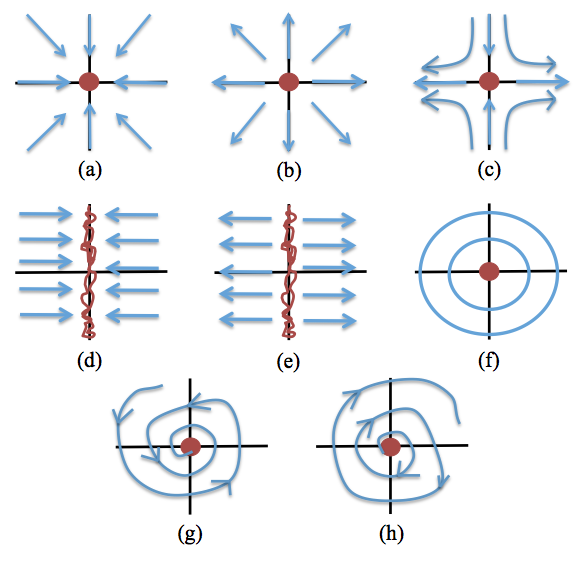
\includegraphics[width=5.0in]{EquilibriaClassification.png}
\caption{Various classifications of equilibrium based on eigenvalues of the Jacobian Matrix. (a) Sink (stable) Equilibrium (b) Source (unstable) Equilibrium (c) Saddle-Point Equilibrium (d) Degenerate Case 1 (e) Degenerate Case 2 (f) Center (g) Stable Foci (h) Unstable Foci}
\label{EquilibriaClassification}
\end{figure}

%
%
% Classifying Equilibria
%
% 
\begin{itemize}
%SINK
\item[ ] {\bf{Sink Equilibrium}}\\

In this case we assume two real eigenvalues, such that $\lambda_1,\lambda_2<0.$\\

 If we imagine finding a ``solution" to our linearized problem, e.g., $\frac{d {\bf{F}}({\bf{x}}_0}{dt} = J({\bf{x}}_0)({\bf{x-x}}_0).$, it is clear we will have the case of decaying exponentials in our diagonalization. Therefore we would assume any trajectory within a neighborhood of the equilibrium, ${\bf{x}}_0$, will head to the equilibria itself. Hence this case is known as a \emph{sink}. It is also stable. \\

This case can be seen in Figure(\ref{EquilibriaClassification})(a). \\

$ $\\


%SOURCE
\item[ ] {\bf{Source Equilibrium}}\\

In this case we assume two real eigenvalues, such that $\lambda_1,\lambda_2>0.$\\

Performing the same thought experiment as above, upon envisioning a solution the linearized problem, we find that any trajectory found within a neighborhood of the equilibrium would point away from the equilibria. Therefore this equilibria is known as a \emph{source}, as all trajectories point away from the equilibrium. It is also deemed unstable.\\

This case can be seen in Figure(\ref{EquilibriaClassification})(b).\\

$ $\\



%SADDLE-POINT
\item[ ] {\bf{Saddle-Point Equilibrium}}\\

In this case we assume two real eigenvalues, such that $\lambda_1>0,\lambda_2<0,$ hence one is positive and one is negative.\\

This case is called a \emph{saddle-point} equilibrium because some trajectories will be pointed towards the equilibria, while others will be pointed away. This is similar the idea of a saddle-point in multivariate calculus. Similarly in multivariate calulus, where a saddle-point is not strictly considered a local maxima or minima, it cannot be deemed either stable or unstable. \\

This case can be seen in Figure(\ref{EquilibriaClassification})(c). \\

$ $\\


%DEGENERATE CASES
\item[ ] {\bf{Degenerate Cases}}\\

In this case we assume two real eigenvalues, such that $\lambda_1\neq0,\lambda_2=0,$ hence one strictly zero and the other is real. In these type of degenerate cases, we will see bifurcated behavior. \\

For the case where $\lambda_1>0$, we believe solutions we act in a manner as seen in Figure(\ref{EquilibriaClassification})(d), while in the case where $\lambda_1<0$, the system has a feel of what is depicted in Figure(\ref{EquilibriaClassification})(e).\\

This type of behavior may be exhibited when radical structural differences occur in the trajectories when perturbing system parameters. \\

$ $\\


%CENETER
\item[ ] {\bf{Centers}}\\

In this case we assume two purely imaginary eigenvalues, such that $\lambda_1=bi,\lambda_2=-bi.$\\ Each trajectory around the equilibria, ${\bf{x}}_0$, is closed and circular in nature. This can be seen in Figure(\ref{EquilibriaClassification})(f). \\

We also note that if the Jaconian is \emph{skew-symmetric} at ${\bf{x}}={\bf{x}}_0$, then the equilbrium will always be a center, i.e., skew-symmetric matrices have purely imaginary eigenvalues. Let's actually do a quick proof.  

\begin{itemize}
\item[ ] {\bf{Proof}}: To show these trajectories are always circular, we begin with the relation that if $A=-A^*$, then the quadratic form $x^* A x = 0$. To prove this we can easily see that,

$$- x^* A x = x^* (-A) x = x^* A^* x = (x^* A x)^* = x^* A x,$$

since the quadratic form is a scalar quantity. Therefore we have $x^* A x = - x^* A x$ and hence $x^* A x = 0.$

Now that we have that relation, we consider the linearization, or actually just a linear system of ODEs,\\
$$\frac{d{\bf{x}}}{dt} = A {\bf{x}}.$$

Consider $A=-A^*$, and multiply the above by ${\bf{x}}^*$, \\

$${\bf{x}}^* \cdot \frac{d{\bf{x}}}{dt} = {\bf{x}}^* A {\bf{x}} = 0$$

Therefore we have \\

$${\bf{x}}^* \cdot \frac{d{\bf{x}}}{dt}  = \frac{1}{2} \frac{d}{dt} ( {\bf{x}}\cdot {\bf{x}} ) = \frac{d}{dt} ||x||^2 = 0.$$

From the above we get that all the orbits must be circular. \\

\end{itemize}

%\begin{Proof}
%To show a matrix has purely imaginary eigenvalues, we start with the \emph{Rayleigh Quotient},
%$$\lambda = \frac{{\bf{x}}^* A{\bf{x}}}{{\bf{x}}^*{\bf{x}}},$$
%%
%where $A\mathbb{R}^N$, ${\bf{x}}$ is our eigenvectors associated with eigenvalue, $\lambda$. Now we take the conjugate transpose (or conjapose...still not catching on? Okay, fine.) of the Rayleigh Quotient to get
%$$\lambda^* = \frac{ {\bf{x}}^* A* {\bf{x}} }{ {\bf{x}}^* {\bf{x}} } = \frac{ {\bf{x}}^* (-A) {\bf{x}} }{ {\bf{x}}^* {\bf{x}} } = -  \frac{ {\bf{x}}^* A {\bf{x}} }{ {\bf{x}}^* {\bf{x}} } = -\lambda.$$
%
%Hence we find that $\lambda^* = -\lambda$ and therefore we get that all eigenvalues must be purely imaginary. 
%\end{Proof}

$ $\\

%STABLE FOCUS
\item[ ] {\bf{Stable and Unstable Foci}}\\

In this case we assume two complex eigenvalues, such that $\lambda_1=a+bi,\lambda_2=a-bi,$ with $b\neq 0.$ \\ 

Depending on the sign of $a$, this system will either spiral towards or away from the equilbrium point. In both cases it will oscillate about the equilibrium with period $b$. Thinking of the solutions to the linearized problem, we note the stability will be controlled by if the solutions decay, i.e., $a<0$, or when they grow uncontrollably, i.e., $a>0.$ \\


For the case when $a<0$, the trajectories spiral towards the equilibria. We call the equilibrium a \emph{stable focus}.  Converging towards the equilibrium point is clear since the real part of the eigenvalue is negative. As in the \emph{sink} case, which also has negative real part, we expect trajectories to flow towards the equilibria. This can be seen in Figure(\ref{EquilibriaClassification})(g). \\

For the case when $a>0$, the trajectories spiral away from the equilibria. We call the equilibrium an \emph{unstable focus}. It is unstable since the real part of the eigenvalue is positive, and hence solutions should flow away from the equilibria, analogous to the \emph{source} case. This can be seen in Figure(\ref{EquilibriaClassification})(h). \\

\end{itemize}

In a neighborhood of the equilibria, we expect the solutions to behave like one of the above cases. Remember this is all \emph{local} analysis and at this junction cannot say anything about global solution behavior...yet  \\